\documentclass[10pt, letterpaper]{article}

%% Packages %%
\usepackage[left=2cm,top=3cm,right=2cm,bottom=2cm]{geometry}
\usepackage{graphicx}
\usepackage[spanish]{babel}
\usepackage[latin1]{inputenc}
\usepackage{amsmath, amsfonts, amssymb, amsthm}
\usepackage{array, xcolor}
\usepackage{chngcntr}
\usepackage{pdfpages}

%% Document format %%
\pagestyle{myheadings}       % Uncomment if don't want page numbers
% \markright{ICE3413 - Hormigon armado avanzado}
\linespread{1.0}
\setlength{\parindent}{0pt}

%% Comandos %%
\definecolor{lightgray}{gray}{0.8}
\newcommand\VRule{\color{lightgray}\vrule width 0.5pt}
\newcommand{\extend}[2]{#1 \hfill #2}
\newcommand{\extendbf}[2]{\textbf{#1 \hfill #2}}
\newcommand{\cm}{\mbox{ cm}}
\newcommand{\ton}{\mbox{ ton}}
\newcommand{\kgcm}{\frac{\mbox{kg}}{\mbox{cm}^2}}
\newcommand{\toncm}{\frac{\mbox{ton}}{\mbox{cm}^2}}
\newcommand{\tonm}{\mbox{ ton-m}}


\title{Tarea 02}
\author{Nicol�s A. Pe�a Escarpentier}
\date{} 

\begin{document}
\maketitle

\section*{Pregunta 1}

\subsubsection*{Escena 1: The Interrogation Chamber}
\begin{enumerate}
\item Los sonidos se encuentran fuera de la cabeza, alrededor mio. Dependiendo de la posici�n del locutor, el efecto que produce, ya que soy capaz de localizar a la fuente del sonido, independiente de la posici�n en la que se encuentra.
\item Percibo la sensaci�n de encontrarme en un lugar encerrado, probablemente con paredes de metal. Da esta sensaci�n por el eco que producen las voces y objetos. Dentro de la habitaci�n no hay muchas cosas: otro prisionero atr�s a la izquierda, objetos de tortura atr�s a la derecha y unas mesas alrededor mio. Adem�s, hay 2 o 3 puertas en la habitaci�n: Una al frente a la derecha, otra al lado derecho (que podr�a ser la misma que la primera) y otra a la izquierda.
\item La escena es muy realista respecto al espacio. Se percibe ampliamente el espacio, otorgando una sensaci�n de profundidad del lugar. Esto se mantiene, ya que la cabeza permanece quieta, al moverla esta sensaci�n se ve apagada.
\item S�, en todos los puntos del espacio pude saber en cierta medida donde se encuentran las cosas o los locutores. El �nico problema era cuando estaban en frente o atr�s mio, ya que al no poder mover la cabeza, no pod�a discernir su posici�n. 
\end{enumerate}

\subsubsection*{Escena 2: Virtual Barber Shop}
\begin{enumerate}
\item Los sonidos se encuentran fuera de la cabeza, alrededor mio. Dependiendo de la posici�n del locutor, el efecto que produce, ya que soy capaz de localizar a la fuente del sonido, independiente de la posici�n en la que se encuentra.
\item El espacio que se perciba es muy realista. Se siente como una sala con pisos y murallas de madera, gracias al eco de los pasos y como se escucha cuando corren la silla. 
\item Esta escena tambi�n es muy realista respecto al espacio. Nuevamente, se disminuye (o niega) el efecto si se mueve la cabeza.
\item S�, el efecto vuelve a ser bastante parejo. En esta escena no permanece tanto tiempo delante o detr�s de la persona, y cuando lo hace lo acompa�a dici�ndolo, lo que ayuda a la percepci�n. Adem�s, el efecto de la bolsa sobre la cabeza es muy convincente.
\end{enumerate}

\section*{Pregunta 2}
El efecto Haas es un efecto psicoac�stico, en el cual si tenemos una se�al de audio, seguida por se�ales m�s d�biles en un intervalo bastante peque�o (para que no se sienta como un eco), el cerebro ``suprime'' las se�ales m�s d�biles, puesto que entiende que son parte de la resonancia de la primera. Adem�s, mediante la diferencia entre el tiempo de llegada a cada o�do, el cerebro es capaz de estimar la posici�n de la fuente de sonido, el tipo de lugar en el que nos encontramos, etc.\\

Otro efecto que busca lo mismo es el \textit{panning}. Mediante cambios en la intensidad del sonido en cada canal, se puede apreciar un cambio en el lugar del instrumento. Pero este efecto no es igual de efectivo que el efecto de precedencia. Adem�s, al usar \textit{panning} el sonido pierde intensidad, mientras que con el efecto estudiado, mantiene su intensidad en todo momento.\\

El experimento realizado consiste en realizar un \textit{patch} en Pure Data, el cual manda una se�al en pulsos repetitivos a los cuales se les aplica un retraso para modelar este efecto. Primero se puso la se�al centrada, para luego ir aplicando el retraso a cada salida (izquierda o derecha). Seg�n las recomendaciones del video visto, el retraso va de $0.1$ a $0.7$ ms. Al realizar este experimento, y sin haber dicho nada a las personas anteriormente, autom�ticamente detectaban que el sonido proven�a de alguno de los lados. A continuaci�n, presento una captura de pantalla del \textit{patch} y \textbf{subpatches} utilizados.

\begin{figure}[h!]
\centering
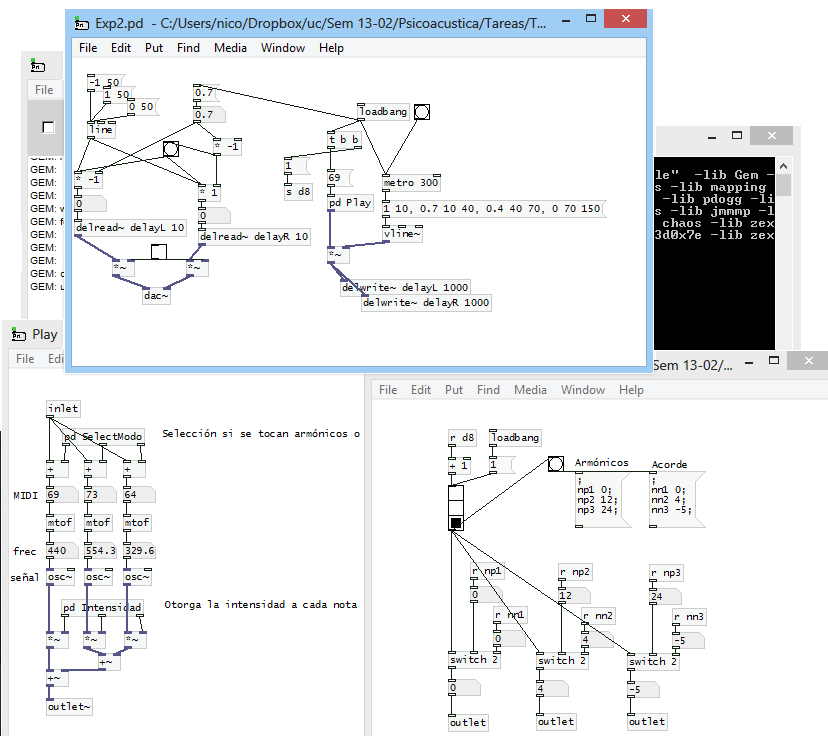
\includegraphics[width=\textwidth]{patches.png}
\caption{Patch de PureData utilizado en el experimento}
\end{figure}

\end{document}